\PassOptionsToPackage{unicode=true}{hyperref} % options for packages loaded elsewhere
\PassOptionsToPackage{hyphens}{url}
%
\documentclass[]{article}
\usepackage{lmodern}
\usepackage{amssymb,amsmath}
\usepackage{ifxetex,ifluatex}
\usepackage{fixltx2e} % provides \textsubscript
\ifnum 0\ifxetex 1\fi\ifluatex 1\fi=0 % if pdftex
  \usepackage[T1]{fontenc}
  \usepackage[utf8]{inputenc}
  \usepackage{textcomp} % provides euro and other symbols
\else % if luatex or xelatex
  \usepackage{unicode-math}
  \defaultfontfeatures{Ligatures=TeX,Scale=MatchLowercase}
\fi
% use upquote if available, for straight quotes in verbatim environments
\IfFileExists{upquote.sty}{\usepackage{upquote}}{}
% use microtype if available
\IfFileExists{microtype.sty}{%
\usepackage[]{microtype}
\UseMicrotypeSet[protrusion]{basicmath} % disable protrusion for tt fonts
}{}
\IfFileExists{parskip.sty}{%
\usepackage{parskip}
}{% else
\setlength{\parindent}{0pt}
\setlength{\parskip}{6pt plus 2pt minus 1pt}
}
\usepackage{hyperref}
\hypersetup{
            pdftitle={Simulation studies: TLP, BLP, and extensions of BLP},
            pdfauthor={Nutcha Wattanachit},
            pdfborder={0 0 0},
            breaklinks=true}
\urlstyle{same}  % don't use monospace font for urls
\usepackage[margin=1in]{geometry}
\usepackage{graphicx,grffile}
\makeatletter
\def\maxwidth{\ifdim\Gin@nat@width>\linewidth\linewidth\else\Gin@nat@width\fi}
\def\maxheight{\ifdim\Gin@nat@height>\textheight\textheight\else\Gin@nat@height\fi}
\makeatother
% Scale images if necessary, so that they will not overflow the page
% margins by default, and it is still possible to overwrite the defaults
% using explicit options in \includegraphics[width, height, ...]{}
\setkeys{Gin}{width=\maxwidth,height=\maxheight,keepaspectratio}
\setlength{\emergencystretch}{3em}  % prevent overfull lines
\providecommand{\tightlist}{%
  \setlength{\itemsep}{0pt}\setlength{\parskip}{0pt}}
\setcounter{secnumdepth}{0}
% Redefines (sub)paragraphs to behave more like sections
\ifx\paragraph\undefined\else
\let\oldparagraph\paragraph
\renewcommand{\paragraph}[1]{\oldparagraph{#1}\mbox{}}
\fi
\ifx\subparagraph\undefined\else
\let\oldsubparagraph\subparagraph
\renewcommand{\subparagraph}[1]{\oldsubparagraph{#1}\mbox{}}
\fi

% set default figure placement to htbp
\makeatletter
\def\fps@figure{htbp}
\makeatother

\usepackage{booktabs}
\usepackage{tabularx}
\usepackage{hyperref}
\usepackage{multicol}
\usepackage{longtable}
\usepackage{array}
\usepackage{multirow}
\usepackage{wrapfig}
\usepackage{float}
\usepackage{colortbl}
\usepackage{pdflscape}
\usepackage{tabu}
\usepackage{threeparttable}
\usepackage{threeparttablex}
\usepackage{makecell}
\usepackage{xcolor}
\usepackage{booktabs}
\usepackage{longtable}
\usepackage{array}
\usepackage{multirow}
\usepackage{wrapfig}
\usepackage{float}
\usepackage{colortbl}
\usepackage{pdflscape}
\usepackage{tabu}
\usepackage{threeparttable}
\usepackage{threeparttablex}
\usepackage[normalem]{ulem}
\usepackage{makecell}
\usepackage{xcolor}

\title{Simulation studies: TLP, BLP, and extensions of BLP}
\author{Nutcha Wattanachit}
\date{8/25/2020}

\begin{document}
\maketitle

\hypertarget{simulation-studies}{%
\section{Simulation studies}\label{simulation-studies}}

The data generating process for the observation \(Y\) in the regression
model is

\[
Y = X_0+a_1X_1+a_2X_2+a_3X_3+ \epsilon, \\
\epsilon \sim(0,1)
\]

where \(a_1,a_2,\) and \(a_3\) are real constants that vary across
different simulation studies, and \(X_0,X_1,X_2,X_3,\) and \(\epsilon\)
are independent, standard normal random variables. The individual
predictive densities have partial access of the above set of covariates.
\(f_1\) has access to only \(X_0\) and \(X_1\), \(f_2\) has access to
only \(X_0\) and \(X_2\), and \(f_3\) has access to only \(X_0\) and
\(X_3\). We want to combine \(f_1,f_2,\) and \(f_3\) to predict \(Y\).
In this setup, \(X_0\) represent shared information, while other
covariates represent information unique to each individual model.

We estimate the pooling/combination formulas on a random sample
\({(f_{1i} , f_{2i} , f_{3i}, Y_i) : i = 1,..., n}\) of size
\(n = 50,000\) and evaluate on an independent test sample of the same
size.

\clearpage

\hypertarget{scenario-1-unbiased-and-calibrated-components}{%
\subsection{Scenario 1: Unbiased and calibrated
components}\label{scenario-1-unbiased-and-calibrated-components}}

In this scenario, \(a_1 = a_2 = 1\) and \(a_3 = 1.1\), so that \(f_3\)
is a more concentrated, sharper density forecast than \(f_1\) and
\(f_2\) (Gneiting and Ranjan (2013)) and they are defined as follows:

\[
\begin{aligned}
f_1&=\text{N}(X_0+a_1X_1,1+a^2_2+a^2_3)\\
f_2&=\text{N}(X_0+a_2X_2,1+a^2_1+a^2_3)\\
f_3&=\text{N}(X_0+a_3X_3,1+a^2_1+a^2_2)\\
\end{aligned}
\]

\begin{table}[!h]
\caption{\label{tab:unnamed-chunk-3}Model Parameters and Log Score}

\centering
\begin{tabular}[t]{lrrrrrr}
\toprule
  & w1 & w2 & w3 & alpha & beta & ncp\\
\midrule
\rowcolor{gray!6}  TLP & 0.267 & 0.259 & 0.474 & NA & NA & NA\\
BLP & 0.298 & 0.292 & 0.410 & 1.464 & 1.459 & NA\\
\rowcolor{gray!6}  nBLP & 0.298 & 0.292 & 0.410 & 1.462 & 1.461 & 0.009\\
cBLP & 0.298 & 0.293 & 0.409 & 1.457 & 1.457 & NA\\
\bottomrule
\end{tabular}
\centering
\begin{tabular}[t]{lrr}
\toprule
\rowcolor{gray!6}    & Training & \vphantom{1} Test\\
\midrule
f1 & -2.001 & -2.004\\
\rowcolor{gray!6}  f2 & -2.001 & -2.008\\
f3 & -1.965 & -1.966\\
\rowcolor{gray!6}  TLP & -1.908 & -1.910\\
BLP & -1.865 & -1.870\\
\addlinespace
\rowcolor{gray!6}  nBLP & -1.865 & -1.870\\
cBLP & -1.865 & -1.870\\
\bottomrule
\end{tabular}
\centering
\begin{tabular}[t]{lrr}
\toprule
\rowcolor{gray!6}    & Training & Test\\
\midrule
f1 & 0.083 & 0.083\\
\rowcolor{gray!6}  f2 & 0.083 & 0.084\\
f3 & 0.083 & 0.083\\
\rowcolor{gray!6}  TLP & 0.064 & 0.064\\
BLP & 0.083 & 0.083\\
\addlinespace
\rowcolor{gray!6}  nBLP & 0.083 & 0.083\\
cBLP & 0.083 & 0.083\\
\bottomrule
\end{tabular}
\end{table}

\begin{figure}[H]

{\centering 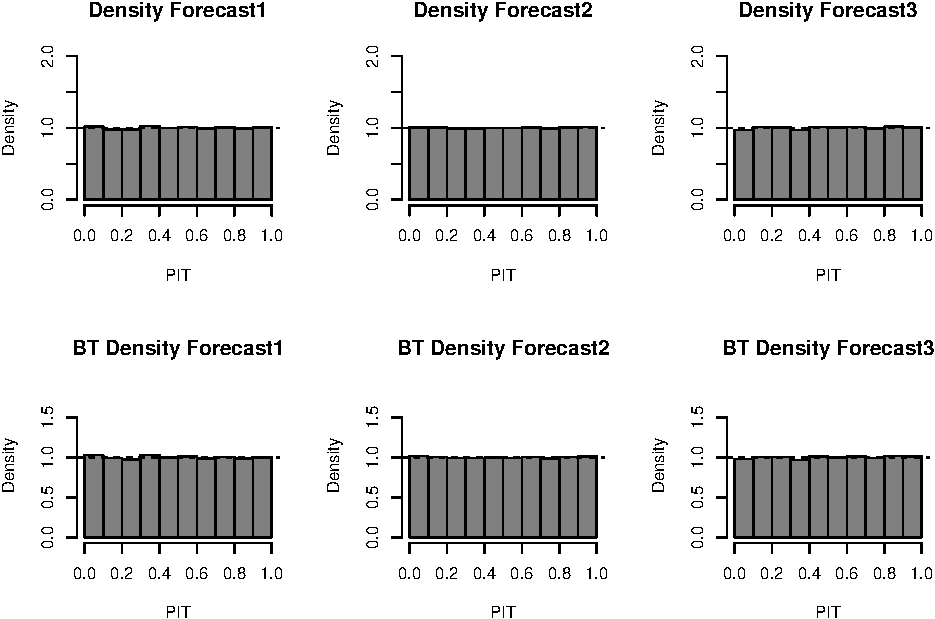
\includegraphics{Newest_BLPsim_new_files/figure-latex/unnamed-chunk-4-1} 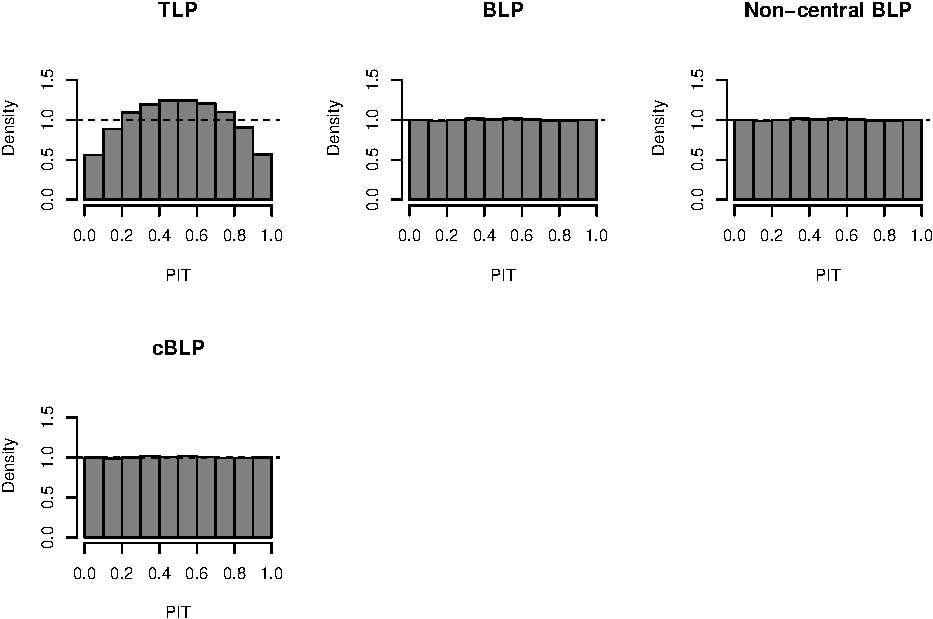
\includegraphics{Newest_BLPsim_new_files/figure-latex/unnamed-chunk-4-2} 

}

\end{figure}

\clearpage

\hypertarget{scenario-2-underdispersed-components}{%
\subsection{Scenario 2 : Underdispersed
components}\label{scenario-2-underdispersed-components}}

We subtract constants from the variances of component density forecasts
as follows:

\[
\begin{aligned}
f_1&=\text{N}(X_0+a_1X_1,(1+a^2_2+a^2_3)-1)\\
f_2&=\text{N}(X_0+a_2X_2,(1+a^2_1+a^2_3)-1)\\
f_3&=\text{N}(X_0+a_3X_3,(1+a^2_1+a^2_2)-1.5)\\
\end{aligned}
\]

\begin{table}[!h]
\caption{\label{tab:unnamed-chunk-7}Model Parameters and Log Score}

\centering
\begin{tabular}[t]{lrrrrrr}
\toprule
  & w1 & w2 & w3 & alpha & beta & ncp\\
\midrule
\rowcolor{gray!6}  TLP & 0.311 & 0.307 & 0.382 & NA & NA & NA\\
BLP & 0.315 & 0.312 & 0.373 & 1.039 & 1.035 & NA\\
\rowcolor{gray!6}  nBLP & 0.315 & 0.312 & 0.373 & 1.037 & 1.036 & 0.01\\
cBLP & 0.278 & 0.272 & 0.450 & 1.455 & 1.455 & NA\\
\bottomrule
\end{tabular}
\centering
\begin{tabular}[t]{lrr}
\toprule
\rowcolor{gray!6}    & Training & \vphantom{1} Test\\
\midrule
f1 & -2.040 & -2.044\\
\rowcolor{gray!6}  f2 & -2.040 & -2.051\\
f3 & -2.115 & -2.116\\
\rowcolor{gray!6}  TLP & -1.876 & -1.881\\
BLP & -1.876 & -1.880\\
\addlinespace
\rowcolor{gray!6}  nBLP & -1.876 & -1.880\\
cBLP & -1.865 & -1.869\\
\bottomrule
\end{tabular}
\centering
\begin{tabular}[t]{lrr}
\toprule
\rowcolor{gray!6}    & Training & Test\\
\midrule
f1 & 0.101 & 0.101\\
\rowcolor{gray!6}  f2 & 0.101 & 0.101\\
f3 & 0.116 & 0.116\\
\rowcolor{gray!6}  TLP & 0.080 & 0.080\\
BLP & 0.082 & 0.082\\
\addlinespace
\rowcolor{gray!6}  nBLP & 0.082 & 0.082\\
cBLP & 0.083 & 0.083\\
\bottomrule
\end{tabular}
\end{table}

\clearpage

\begin{figure}[H]

{\centering 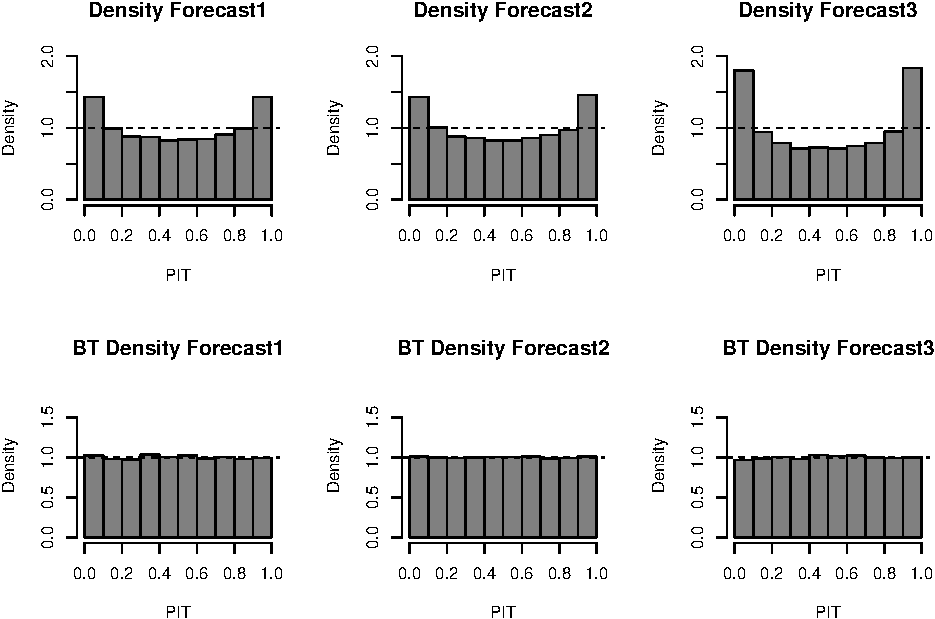
\includegraphics{Newest_BLPsim_new_files/figure-latex/unnamed-chunk-8-1} 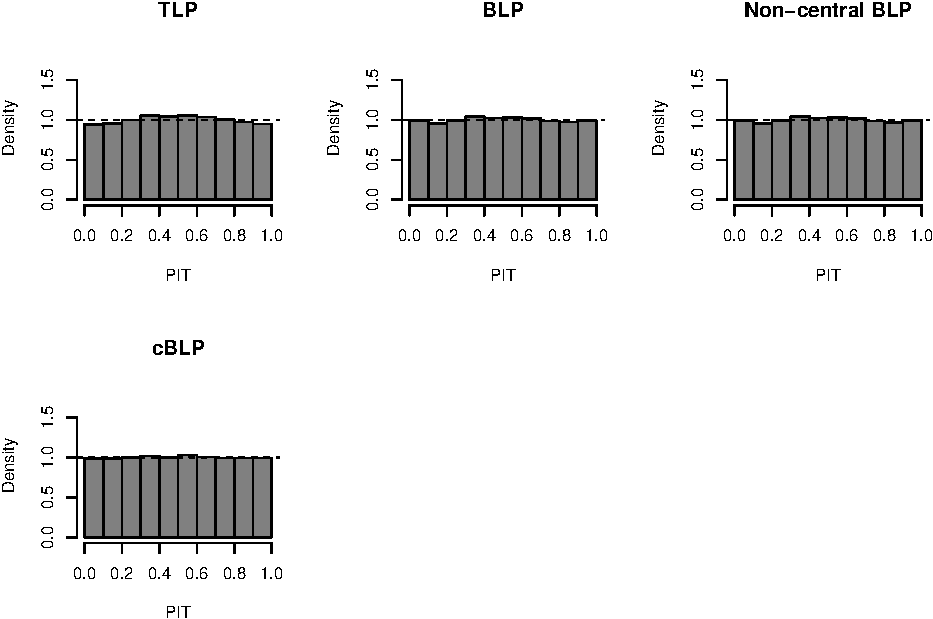
\includegraphics{Newest_BLPsim_new_files/figure-latex/unnamed-chunk-8-2} 

}

\end{figure}

\clearpage

\hypertarget{scenario-3-overdispersed-components}{%
\subsection{Scenario 3: Overdispersed
components}\label{scenario-3-overdispersed-components}}

We add constants from the variances of component density forecasts as
follows:

\[
\begin{aligned}
f_1&=\text{N}(X_0+a_1X_1,(1+a^2_2+a^2_3)+2)\\
f_2&=\text{N}(X_0+a_2X_2,(1+a^2_1+a^2_3)+2)\\
f_3&=\text{N}(X_0+a_3X_3,(1+a^2_1+a^2_2)+2)\\
\end{aligned}
\]

\begin{table}[!h]
\caption{\label{tab:unnamed-chunk-11}Model Parameters and Log Score}

\centering
\begin{tabular}[t]{lrrrrrr}
\toprule
  & w1 & w2 & w3 & alpha & beta & ncp\\
\midrule
\rowcolor{gray!6}  TLP & 0.220 & 0.209 & 0.571 & NA & NA & NA\\
BLP & 0.297 & 0.291 & 0.412 & 2.145 & 2.138 & NA\\
\rowcolor{gray!6}  nBLP & 0.297 & 0.291 & 0.412 & 2.143 & 2.140 & 0.01\\
cBLP & 0.301 & 0.295 & 0.404 & 1.455 & 1.455 & NA\\
\bottomrule
\end{tabular}
\centering
\begin{tabular}[t]{lrr}
\toprule
\rowcolor{gray!6}    & Training & \vphantom{1} Test\\
\midrule
f1 & -2.052 & -2.053\\
\rowcolor{gray!6}  f2 & -2.051 & -2.056\\
f3 & -2.022 & -2.022\\
\rowcolor{gray!6}  TLP & -2.006 & -2.008\\
BLP & -1.861 & -1.865\\
\addlinespace
\rowcolor{gray!6}  nBLP & -1.861 & -1.865\\
cBLP & -1.866 & -1.870\\
\bottomrule
\end{tabular}
\centering
\begin{tabular}[t]{lrr}
\toprule
\rowcolor{gray!6}    & Training & Test\\
\midrule
f1 & 0.062 & 0.062\\
\rowcolor{gray!6}  f2 & 0.062 & 0.063\\
f3 & 0.061 & 0.061\\
\rowcolor{gray!6}  TLP & 0.049 & 0.049\\
BLP & 0.083 & 0.084\\
\addlinespace
\rowcolor{gray!6}  nBLP & 0.083 & 0.084\\
cBLP & 0.083 & 0.083\\
\bottomrule
\end{tabular}
\end{table}

\clearpage

\begin{figure}[H]

{\centering 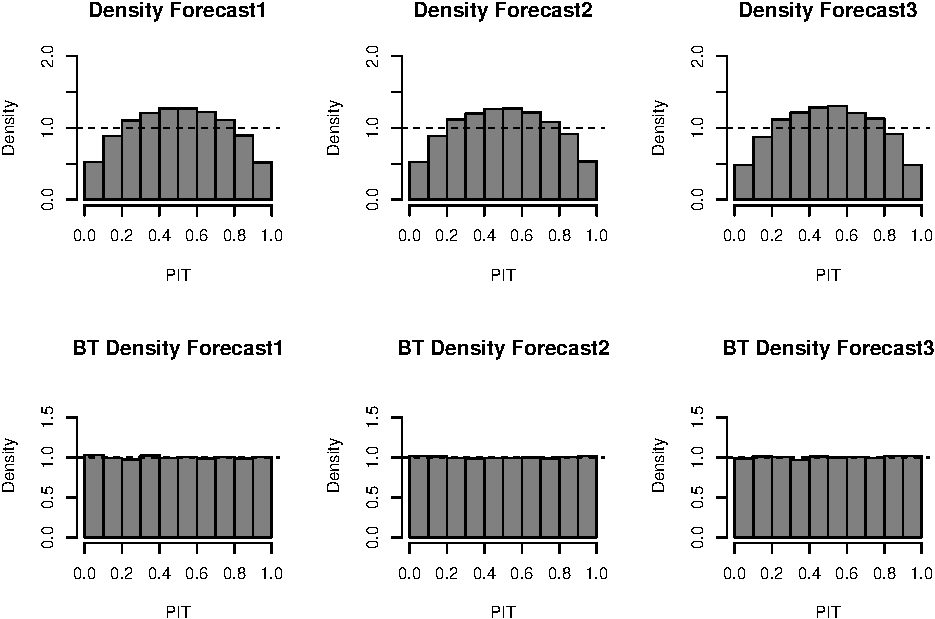
\includegraphics{Newest_BLPsim_new_files/figure-latex/unnamed-chunk-12-1} 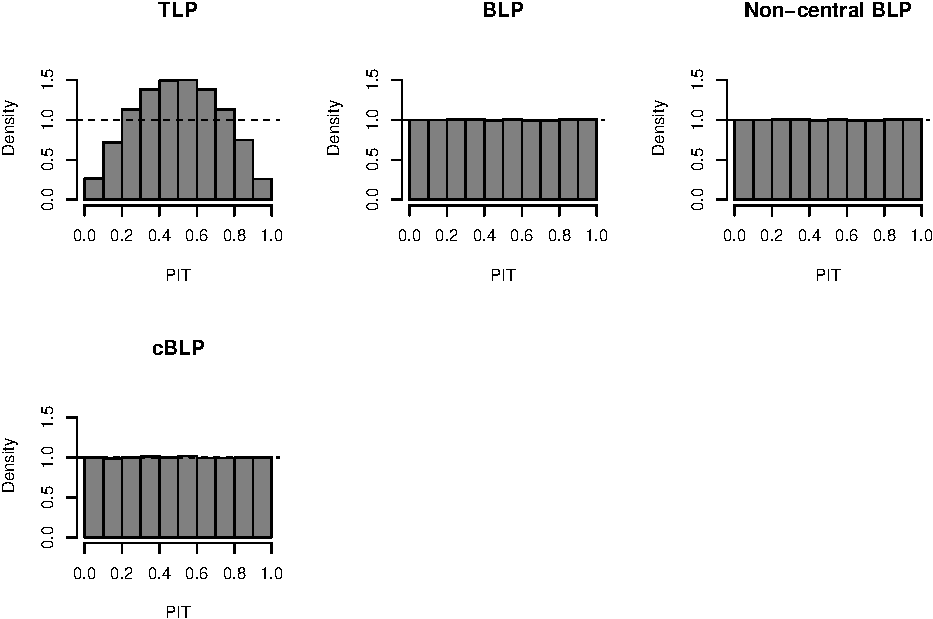
\includegraphics{Newest_BLPsim_new_files/figure-latex/unnamed-chunk-12-2} 

}

\end{figure}

\clearpage

\hypertarget{scenario-4-over--and-underdispersed-components}{%
\subsection{Scenario 4: Over- and underdispersed
components}\label{scenario-4-over--and-underdispersed-components}}

The models are defined as follows:

\[
\begin{aligned}
f_1&=\text{N}(X_0+a_1X_1,(1+a^2_2+a^2_3)-0.8)\\
f_2&=\text{N}(X_0+a_2X_2,(1+a^2_1+a^2_3)+0.6)\\
f_3&=\text{N}(X_0+a_3X_3,(1+a^2_1+a^2_2)-1)\\
\end{aligned}
\]

\begin{table}[!h]
\caption{\label{tab:unnamed-chunk-15}Model Parameters and Log Score}

\centering
\begin{tabular}[t]{lrrrrrr}
\toprule
  & w1 & w2 & w3 & alpha & beta & ncp\\
\midrule
\rowcolor{gray!6}  TLP & 0.335 & 0.191 & 0.474 & NA & NA & NA\\
BLP & 0.288 & 0.333 & 0.379 & 1.287 & 1.280 & NA\\
\rowcolor{gray!6}  nBLP & 0.288 & 0.333 & 0.379 & 1.285 & 1.283 & 0.015\\
cBLP & 0.345 & 0.198 & 0.456 & 1.436 & 1.436 & NA\\
\bottomrule
\end{tabular}
\centering
\begin{tabular}[t]{lrr}
\toprule
\rowcolor{gray!6}    & Training & \vphantom{1} Test\\
\midrule
f1 & -2.032 & -2.024\\
\rowcolor{gray!6}  f2 & -2.012 & -2.011\\
f3 & -2.017 & -2.007\\
\rowcolor{gray!6}  TLP & -1.893 & -1.887\\
BLP & -1.877 & -1.871\\
\addlinespace
\rowcolor{gray!6}  nBLP & -1.877 & -1.871\\
cBLP & -1.874 & -1.867\\
\bottomrule
\end{tabular}
\centering
\begin{tabular}[t]{lrr}
\toprule
\rowcolor{gray!6}    & Training & Test\\
\midrule
f1 & 0.097 & 0.097\\
\rowcolor{gray!6}  f2 & 0.076 & 0.076\\
f3 & 0.102 & 0.102\\
\rowcolor{gray!6}  TLP & 0.074 & 0.073\\
BLP & 0.083 & 0.082\\
\addlinespace
\rowcolor{gray!6}  nBLP & 0.083 & 0.082\\
cBLP & 0.082 & 0.082\\
\bottomrule
\end{tabular}
\end{table}

\clearpage

\begin{figure}[H]

{\centering 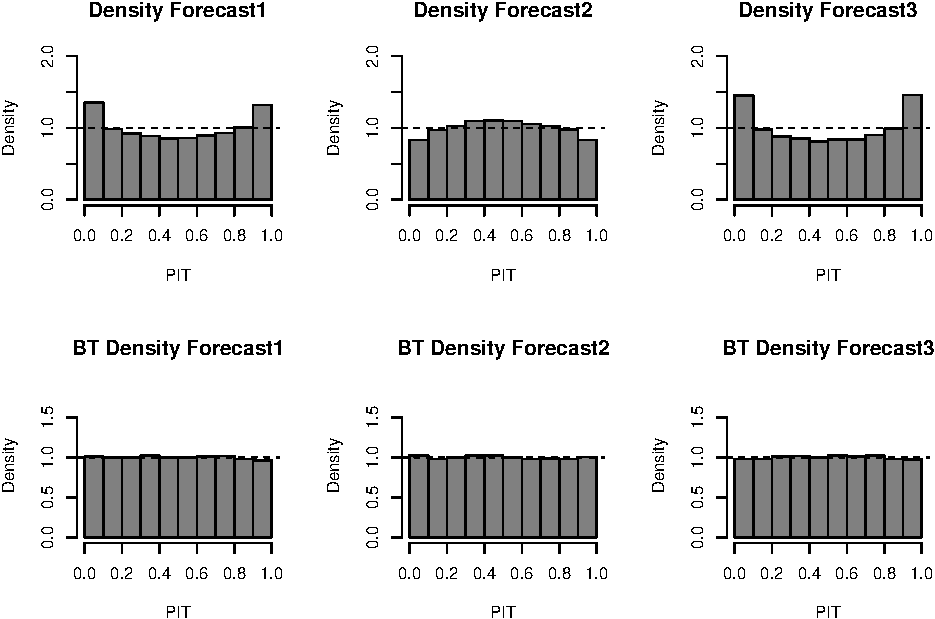
\includegraphics{Newest_BLPsim_new_files/figure-latex/unnamed-chunk-16-1} 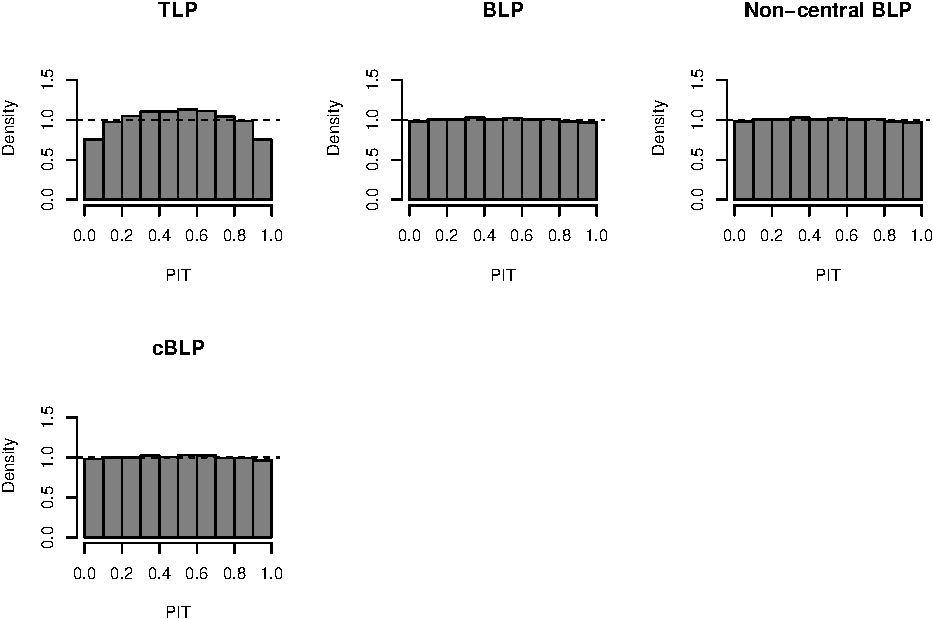
\includegraphics{Newest_BLPsim_new_files/figure-latex/unnamed-chunk-16-2} 

}

\end{figure}

\hypertarget{comments}{%
\subsection{Comments}\label{comments}}

\begin{itemize}
\tightlist
\item
  BLP, nBLP, and cBLP outperforms TLP based on log score and
  probabilistic calibration in most scenarios.
\item
  cBLP does better when all or most components are underdispersed. The
  last scenario where the sharpest component is underdispersed cBLP also
  does well probably because it's able to fix the dispersion of the
  sharp component and then assign the most weight to that component.
\end{itemize}

\end{document}
